\section{Second-order nonlinear time-invariant systems}
We first consider the system
\begin{equation}
\begin{array}{l}{\dot{x}_{1}=f_{1}\left(x_{1}, x_{2}\right)} \\ {\dot{x}_{2}=f_{2}\left(x_{1}, x_{2}\right)}\end{array}
\end{equation}

\textbf{Phase-plane analysis:} Determine the system behavior by constructing a phase portrait, i.e. plotting different IVP solutions in the phase space.

\textbf{Local analysis:}
\begin{itemize}[topsep=0pt]
    \item Linearize about $x^*$.
    \item Find egeinvalues $\lambda(A)$.
    \item Classify equilibrium points for $f(x^*) = 0$.
    If $\lambda$ is real, them we either get a stable node ($\lambda_2 < \lambda_1 < 0$), unstable node ($0 < \lambda_2 < \lambda_1$) or a saddle point ($\lambda_2 < 0 < \lambda_1$).
    In the complex case $\lambda_{1,2} = \alpha \pm \beta i$, then we either get a center focus ($\alpha = 0$), a stable focus ($\alpha < 0$) or an unstable focus ($\alpha > 0$).
\end{itemize}

\begin{figure}[!htb]
    \centering
    \begin{subfigure}{0.3\textwidth}
        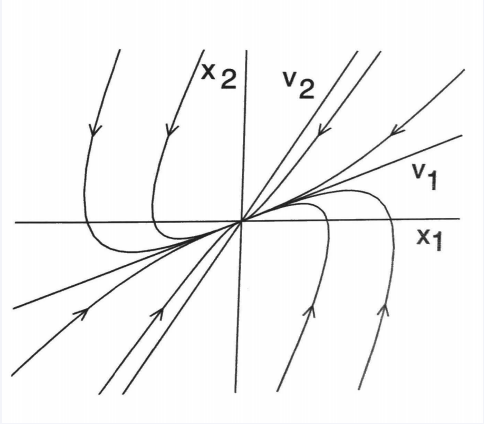
\includegraphics[height=3cm]{figures/sn.png}
        \caption{Stable node}
    \end{subfigure}
    \begin{subfigure}{0.3\textwidth}
        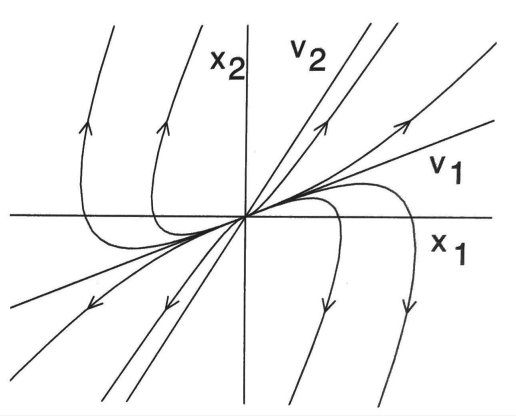
\includegraphics[height=3cm]{figures/un.png}
        \caption{Unstable node}
    \end{subfigure}
    \begin{subfigure}{0.3\textwidth}
        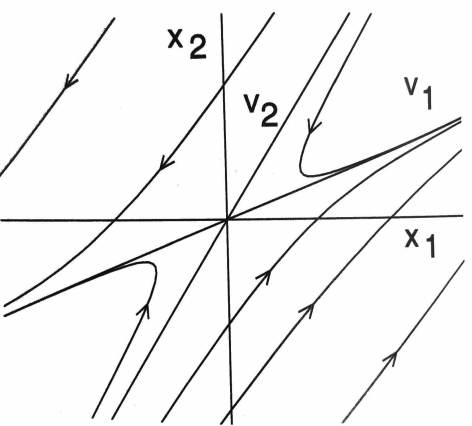
\includegraphics[height=3cm]{figures/sp.png}
        \caption{Saddle point}
    \end{subfigure}
    \label{fig:phase_portraits1}
\end{figure}

\begin{figure}[!htb]
    \centering
    \begin{subfigure}{0.3\textwidth}
        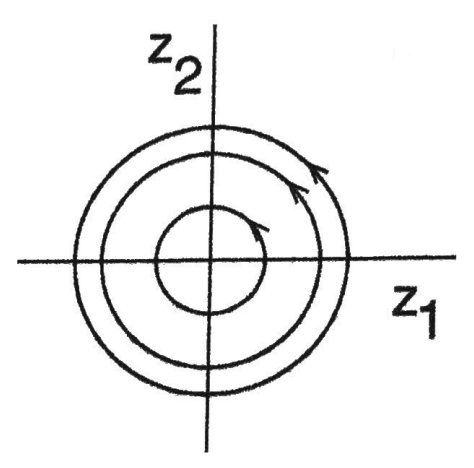
\includegraphics[height=3cm]{figures/cf.png}
        \caption{Center focus}
    \end{subfigure}
    \begin{subfigure}{0.3\textwidth}
        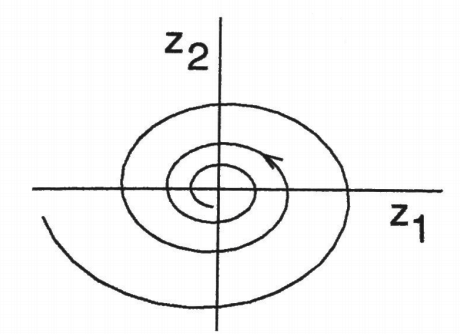
\includegraphics[height=3cm]{figures/sf.png}
        \caption{Stable focus}
    \end{subfigure}
    \begin{subfigure}{0.3\textwidth}
        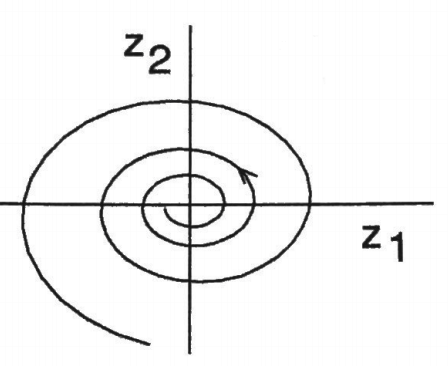
\includegraphics[height=3cm]{figures/uf.png}
        \caption{Unstable focus}
    \end{subfigure}
    \label{fig:phase_portraits2}
\end{figure}

\textbf{Topological equivalence:} if the real part of the eigenvalues are nonzero, then the local phase-portrait corresponds to the phase portrait of the linearized system.

\subsection{Periodic orbits and limit cycles}
\begin{definition}
    Periodic orbit: $\exists T>0$ s.t. $x(t+T)=x(t) \quad \forall t \geq 0$.
\end{definition}
\begin{definition}
    Limit cycle: non-trivial isolated periodic orbit.
\end{definition}
\begin{lemma}
    Poincaré-Bendixson criterion:\\
    Let $M$ be a closed bounded subset of the plane s.t.:
    \begin{itemize}[topsep=0pt]
        \item $M$ contains no $x^*$, or it
        contains only one $x^*$ with the property that
        the eigenvalues of the Jacobian matrix at $x^*$ have
        positive real parts (unstable focus or unstable node).
        \item Every trajectory starting in M stays in M $\forall t>t_0$.
    \end{itemize}
    Then $M$ contains a periodic orbit of the system.
\end{lemma}

\begin{lemma}
    Bendixson negative criterion:\\
    If on a simply connected region $D$,$\frac{\partial f_{1}}{\partial x_{1}}+\frac{\partial f_{2}}{\partial x_{2}}$ is not identically zero and does not change sign, then the
    system has no periodic orbits lying entirely in $D$.
\end{lemma}

\begin{corollary}
    $C$ is a periodic orbit $\implies \Sigma_i I = 1$ (sum of indeces of equilibrium points in $C$, where saddle points have index -1 and others have index 1)
\end{corollary}

\section{Fundamental properties}
\textbf{Lipschitz:} $\|f(t, x)-f(t, y)\| \leq L\|x-y\|$ \\
Either locally Lipschitz on $\mathbb{D}$ (L varies), Lipschitz in $\mathbb{D}$ or globally Lipschitz.

\begin{theorem}
    Local existence and uniqueness:\\
    If
    \begin{itemize}[topsep=0pt]
        \item $f(t, x)$ is piecewise continuous in $t$,
        \item $f(t, x)$ is Lipschitz $\forall x, y \in B=\left\{x \in \mathbb{R}^{n} |\left\|x-x_{0}\right\| \leq r\right\} \forall t \in\left[t_{0}, t_{1}\right]$,
    \end{itemize}
    Then there exists a unique solution of the IVP $x(t)$
    on $t \in\left[t_{0}, t_{0}+\delta\right]$.
\end{theorem}

\section{Lyapunov stability}
\subsection{Stability of equilibrium points}
\textbf{Asymptotic stabilization problem:}
Find $\gamma(t, e)$ s.t. $e=0$ is an asymptotically stable equilibrium point.\\
Regulation vs. trajectory tracking.

\begin{definition}
    Stability: $x=0$ is stable iff
    $\forall \varepsilon>0 \quad \exists \delta(\varepsilon)>0 \quad \text { s.t. } \quad\|x(0)\|<\delta \Rightarrow\|x(t)\|<\varepsilon \quad \forall t \geq 0$
\end{definition}
\begin{definition}
    Asymptotic stability: $x = 0$ is (locally) asymptotically stable iff it is stable, and\\
    $\exists r>0 \quad \text { s.t. } \quad\|x(0)\|<r \Rightarrow \lim _{t \rightarrow \infty} x(t)=0$
\end{definition}
\begin{definition}
    Region of attraction: $B_{r}=\left\{x \in \mathbb{R}^{n}:\|x\|<r\right\}$. We denote $R_A$ as the union of all the regions of attraction.
\end{definition}
\begin{definition}
    Global asymptotic stability: $x = 0$ is GAS iff it is stable, and $\lim_{t \rightarrow \infty} x(t)=0 \quad \forall x(0)$
\end{definition}
\begin{definition}
    Exponential stability: $x = 0$ is exponentially stable iff\\
    $\exists r, k, \lambda>0$ s.t. $\|x(0)\|<r \Rightarrow\|x(t)\| \leq k\|x(0)\| e^{-\lambda t} \quad \forall t \geq 0$
\end{definition}
\begin{definition}
    Global exponential stability: $x = 0$ is GES iff
    $\exists k, \lambda>0$ s.t. $\forall x(0) \quad\|x(t)\| \leq k\|x(0)\| e^{-\lambda t} \quad \forall t \geq 0$
\end{definition}
\begin{remark}
    It is useful to think in terms of stability + convergence to seperate the different stability properties.
\end{remark}

\subsection{Lyapunov's indirect method}
\begin{theorem}
    Lyapunov's indirect method:\\
    Let $x = 0$ be an equilibrium point for
    \begin{equation}
        \dot{x}=f(x), \quad f: \mathbb{D} \subset \mathbb{R}^{n} \rightarrow \mathbb{R}^{n} \quad \text { is } \quad C^{1}
    \end{equation}
    \begin{enumerate}[topsep=0pt]
        \item Linearize about $x=0, \dot{x} = Ax$, where $A=\left.\frac{\partial f}{\partial x}\right|_{x=0}$.
        \item Find the eigenvalues $\lambda_{1}(A), \ldots, \lambda_{n}(A)$.
        \item Categorize the eigenvalues:
        \begin{itemize}[topsep=0pt]
            \item $\forall i \quad \operatorname{Re}\left(\lambda_{i}\right)<0 \Rightarrow$ asymptotically(exponentially) stable
            \item $\exists i \quad \operatorname{Re}\left(\lambda_{i}\right)>0 \Rightarrow$ unstable
            \item $\forall i \quad \operatorname{Re}\left(\lambda_{i}\right)\leq 0 \Rightarrow$ inconclusive
        \end{itemize}
    \end{enumerate}
\end{theorem}
While Lyapunov's indirect method is simple to use, the results are only local and often inconclusive. Let's see if we can do better ey?

\subsection{Lyapunov's direct method}
\begin{definition}
    Lyapunov function:\\
    $V$ is a Lyapunov function for $x=0$ iff
    \begin{itemize}[topsep=0pt]
        \item $V$ is $C^1$
        \item $V(0)=0, \quad V(x)>0 \quad \text { in } \quad \mathbb{D} \backslash\{0\}$
        \item $\dot{V}(0)=0, \quad \dot{V}(x) \leq 0 \quad \text { in } \quad \mathbb{D} \backslash\{0\}$
    \end{itemize}
    If $\dot{V}(x) < 0 \quad \text { in } \quad \mathbb{D} \backslash\{0\}$ then $V$ is a strict Lyapunov function for $x=0$.
\end{definition}

\begin{theorem}
    Lyapunov's stability theorem:
    \begin{itemize}[topsep=0pt]
        \item If $\exists V(x)$ for $x=0$, then $x=0$ is stable.
        \item If $\exists$ strict $V(x)$ for $x=0$, then $x=0$ is asymptotically stable.
    \end{itemize}
\end{theorem}

\begin{theorem}
    Chetaev's instability theorem:\\
    If $\dot{V}(x) > 0$ in a set $U = \{x \in B_r | V(x) > 0\}$, then $x=0$ is unstable.
\end{theorem}

\begin{definition}
    Radially unboundedness: $\| x\| \rightarrow \infty \implies V(x) \rightarrow \infty$
\end{definition}

\begin{theorem}
    If $\exists$ strict  $V : \mathbb{R}^n \rightarrow \mathbb{R}$ for $x=0$ and
    $V$ is radially unbounded,
    then $x=0$ is GAS.
\end{theorem}

\begin{theorem}
    If there exist a function $V : \mathbb{D} \rightarrow \mathbb{R}$ and constants $a, k_1, k_2, k_3 > 0$ s.t.
    \begin{itemize}[topsep=0pt]
        \item $V$ is $C^1$
        \item $k_{1}\|x\|^{a} \leq V(x) \leq k_{2}\|x\|^{a} \quad \forall x \in \mathbb{D}$
        \item $\dot{V}(x) \leq-k_{3}\|x\|^{a} \quad \forall x \in \mathbb{D}$
    \end{itemize}
    then $x=0$ is exponentially stable. If these conditions hold for $\mathbb{D} = \mathbb{R}^n$, then $x=0$ is GES. 
\end{theorem}

\begin{remark}
    $\lambda_{min}(P) \|x\|^2 \leq x^{\top} P x \leq \lambda_{max}(P) \|x\|^2$
\end{remark}

\begin{remark}
    How to deal with indeterminate signs in $\dot{V}$?
    \begin{itemize}[topsep=0pt]
        \item Completion of squares: $x_1 x_2 \leq \frac{1}{2}(x_1^2 + x_2^2)$
        \item Young's inequality: $x_1 x_2 \leq \epsilon x_1^2 + \frac{1}{4\epsilon}x_2^2$
        \item Cauchy-Schwarz' inequality: $\left|a_{1} x_{1}+a_{2} x_{2}+\cdots+a_{n} x_{n}\right| \leq \sqrt{\left(a_{1}^{2}+a_{2}^{2}+\cdots+a_{n}^{2}\right)}\|x\|_{2}$
    \end{itemize}
\end{remark}

\subsection{The invariance principle}
\begin{definition}
    Invariant set: $x(0) \in M \implies x(t) \in M \quad \forall t \in \mathbb{R}$
\end{definition}

\begin{definition}
    Positively invariant set: $x(0) \in M \implies x(t) \in M \quad \forall t \geq 0$
\end{definition}

\begin{definition}
    Level set: $\Omega_{c}=\left\{x \in \mathbb{R}^{n}: V(x) \leq c\right\}$
\end{definition}

\begin{theorem}
    La Salle's theorem:\\
    If $\exists V : \mathbb{D} \rightarrow \mathbb{R}$ s.t.
    \begin{itemize}[topsep=0pt]
        \item $V$ is $C^1$
        \item $\exists c>0 \text { such that } \Omega_{c}=\left\{x \in \mathbb{R}^{n} | V(x) \leq c\right\} \subset \mathbb{D} \text { is bounded }$
        \item $\dot{V}(x) \leq 0 \quad \forall x \in \Omega_{c}$
    \end{itemize}
    Let $E=\left\{x \in \Omega_{c} | \dot{V}(x)=0\right\}$. Let $M$ be the largest invariant set contained in $E$.
    Then $x(0) \in \Omega_{c} \Rightarrow x(t) \stackrel{t \rightarrow \infty}{\longrightarrow} M$.
\end{theorem}

\begin{definition}
    Region of attraction:\\
    Let $x=0$ be an asymptotically stable equilibrium point of the system $\dot{x} = f(x)$, where $f: \mathbb{D} \rightarrow \mathbb{R}^{n}$ is locally Lipschitz and $\mathbb{D} \subset \mathbb{R}^{n}$ contains the origin.
    Let $\phi\left(t, x_{0}\right)$ be the solution. Then the region of attraction is
    \begin{equation}
        R_{A}=\left\{x_{0} \in \mathbb{D} \quad | \quad \phi\left(t, x_{0}\right) \text { is defined } \forall t \geq 0 \text { and } \phi\left(t, x_{0}\right) \rightarrow 0 \text { as } t \rightarrow \infty\right\}
    \end{equation}
\end{definition}
(I.e. all the points with a corresponding solution that converges to the origin).
\begin{remark}
    GAS iff $R_A = \mathbb{R}^n$.
\end{remark}

\textbf{Estimate of $R_A$:} choose the largest set $\Omega_{c}$ in $\mathbb{D}$ which is bounded, and only the connected component of $\Omega_{c}$ that contains the origin.
Then this subset is a subset of $R_A$.

\subsection{Stability analysis of time-variant systems}

\section{Input-to-state stability}
\subsection{Input-to-state stability}
\subsection{Input-output stability}

\section{Passivity}

\section{Nonlinear control}
\subsection{Passivity-based control}
\subsection{Feedback linearization}
\subsection{Adaptive control}
\subsection{Backstepping}